\section{Prime fields}\label{sec:prime}

Over $\FF_p$ there is no subfield to descend to and no Frobenius to fold,
so index calculus must find structure in the factor base itself
(\S\ref{sec:background}). The programme tried known-answer ladders,
root-finding and pair-table oracles, the Petit--Kosters--Messeng Kummer
tower, structured bases on the P-256 field, isogeny-class walks on the NIST
curves, and lattice reformulations. No prime-field arm comes within a
single-digit factor of rho except on the smallest Table~B rows, and the gap
grows with size. The section ends with Gaudry's $k=4$ index calculus over
$\FF_{p^4}$, the one odd-characteristic extension field the programme
measured end to end. Every study is listed in Appendix~\ref{sec:catalogue}.

\subsection{Known-answer ladders and leaderboard rows}

Over prime fields the ledger tracks staged known-answer ladders
(\art{docs/ic/boundary_targets.json}, regime \texttt{prime}). On $j=0$
curves the staged driver recovers a 20-bit logarithm
($p=1{,}048{,}609$) in 56.8--64.9\,s of IC wall against 150--153\,ms of rho
on the identical public point, with split timers and three seeds; running
the relation search on 14 threads made that stage $3$--$4.4\times$ faster in
wall time with counted work unchanged
(\art{research/j0_parallel_relations_20261016/}). On the generic $a=-3$
shape (P-256 and CryptoPro-B class), a Semaev-$\Sem4$ three-decomposition
family with Cantor--Zassenhaus root finding yields one relation per trial at
$p=65{,}519$ with a 120-point base; at fixed base size, median trials per
relation grow from 2 to 28 to 379--506 at 16, 20 and 24 bits, about
$16\times$ per four bits. The prime \texttt{vs\_rho} row is \emph{not
achieved} at any measured size.

Table~B of \art{docs/ic/LEADERBOARD.md} has eight prime rows,
$\log_2 r=9.7$--$23.4$, one target, $m=2$, folded pair table with walked
targets: IC is $6.34$, $5.47$, $6.43$, $6.71$, $5.82$, $8.3$, $10.5$ and
$13.5\times$ matched rho, the ratio rising from about 18 bits. All eight
passed the validation gate on 24 October
(\art{research/ic_validation_gate_20261024/}). In ecbench the root-finding
pair table is $16$--$20\times$ matched rho in counted GAE, and $7.46\times$
$[5.82,9.63]$ with a lane collector, all lower bounds
(\art{research/ecbench_rootfinding_lanes_20261013/}); a planner that picks
the base, stop rule and oracle beat every one-change alternative on six
curves at $w=0$, the root-find-and-subtract variant by $171$--$439\times$
(\art{research/ic_planner_validation_20261020/}). The frontier campaign's
two-summand prime arm goes from $10.5\times$ rho at 20 bits to $102\times$ at
40 bits (\S\ref{sec:campaign}).

\paragraph{Root finding against Buchberger on NIST shapes.} Per query, root
finding of Semaev's $\Sem3$ was $3{,}021\times$ (P-256 shape) to
$5{,}802\times$ (P-224) cheaper than the comparison arm at a six-point base
(\art{research/semaev_rootfind_nist_20261012/}); the arm was
\texttt{groebner\_f4::buchberger}, not F4, so the ratio is against
Buchberger (\S\ref{sec:corrections}). It is an oracle ratio with no complete
solve. A host emulation of a GPU decomposition kernel passed six
configurations on 40--61-bit P-256-class curves
(\art{research/gpu_rootfind_decomposition_20261012/}); no device ran it.
Three frozen SMT formulations of a 20-bit decomposition all returned
\textsc{unknown} at 120\,s, where the native reference needed 146 probes
(\art{research/prime_field_smt_20261005/}).

\paragraph{Earlier, in crypto-autoresearcher.} The first end-to-end
prime-field index calculus of the laboratory predates this repository's:
an imported Autolab round of 1 June 2026 solved logarithms with an $m=3$
Semaev index calculus over a factor base of the smallest valid abscissae, at
a fitted cost exponent of $0.889$ against rho's $0.5$, IC/rho growing from
$21.5$ to $205.7$ over 10--18 bits (\art{ar:experiments/EXP-ALPF-032/analysis.md}).
Structured bases there weakened rather than supported a relation excess
(\art{ar:ledger/evidence/EV-PFDR-f6b76c.yaml}), and on one 13-bit curve an
apparent early fall of the degree fired identically when the Semaev form
was replaced by a random polynomial but not when the factor-base
constraints were, so it came from the factor base, not from the summation
polynomial (\art{ar:experiments/EXP-PFDR-4bfc6f/analysis.md}). A separate repository asked the
underlying question directly---is there any coordinate-defined subset of
$E(\FF_p)$ that interacts with addition better than a random subset?---and
found none on toy curves (\texttt{ecdlp-prime-field-smallness},
\art{README.md} at \texttt{4f20be9b36}).

\subsection{The Kummer tower}\label{sec:pkm}

Petit, Kosters and Messeng's base $V=\mu_{2^t}$ (the roots of
$x^{2^t}-1$) gives prime-field summation systems extra structure for an
algebraic solver. Its claim rests on the solving degree of those systems
staying bounded as $N=m\ell$ grows; the programme measured that degree for
four weeks.

\paragraph{The solving degree.} The pilot found F4's solving degree at
4--5 for $m=2$ through $N=18$ and read the preregistered ``grows like $N$''
as failing at toy size (\art{research/pkm_tower_pilot_20260924/}). Round 2
showed it is not bounded: at $m=2$ it is 5 to $N=18$ and 6 at $N=20,22$, at
$m=3$ it reaches 7 at $N=15$, and the null family behaves the same
(\art{research/pkm_tower_round2_20260925/}). At $m=4$, $N=16$ finished at
$D=7$, as at $N=12$ (\art{research/pkm_tower_round3_20260925/}); at $m=3$
the line reads $6,6,7,7$ over $N=9$--$18$
(\art{research/pkm_tower_round7_20261006/}). Signature engines agreed with
F4 but needed one or two degrees more and $1.7$--$28\times$ the memory, so F4
stayed (rounds 4--5); a full-echelon exit cut multiply-adds $39.8\%$ at
$m=4$, $N=12$ without moving $D$ (round 6). The torus and split Dickson
presentations give the same $D$ in every cell, and the Kummer $D$ does not
depend on the 2-adic valuation (\art{research/pkm_dickson_torus_20261015/}).
At $m=3$, $N=21$ two engines finished every degree-7 step without reaching
the unit ideal and stopped inside degree 8 on memory---the native
\texttt{f4\_fp\_tower} at a 317\,GB matrix cap after a 67\,GB peak, msolve at
99.6\,GiB on 16 threads (\art{research/pkm_lead1_m3n21_20261016/},
\art{research/pkm_m3_n21_msolve_20261018/}). That implies $D\ge8$ at
$N=21$, which both studies read as inconclusive because no degree-8 step
completed. The Certicom-131 programme's gate needs $D\le3$ at $m\ge4$; the
toy plateau at 7 is above it, at $2^{89}$--$2^{98}$ (generous) and
$2^{129}$--$2^{139}$ (plain) at 131 bits
(\art{docs/ic/CERTICOM131_IC_PROGRAM.md}). The exponent sum of decompositions
on the tower is indistinguishable from random at $k=1$--$6$
(\art{research/ic_exponent_falsifiers_20261013/}).

\paragraph{In ecbench.} We ran the tower end to end with the root-finding
oracles on five curves of 20--28 bits (896 runs, all verified, all replay
audits OK; \art{research/pkm_tower_ecbench_20261013/}). Index calculus
costs $34.0$, $41.9$, $29.4$, $96.6$ and $140.6\times$ rho-negation in $S$
(95\% intervals in Figure~\ref{fig:prime}), growing by $0.26\pm0.28$ bits of
$S_{IC}/S_\rho$ per bit of $r$, consistent with the $p^{1/6}$ the floors
predict. The tower base costs the same as a plain base of the same size to
within 1\% (ratios $0.999$--$1.012$): PKM's structure helps an algebraic
solver, not a table. An isogeny-tower variant costs $1.00$--$1.33\times$ the
plain base once its auxiliary-curve search is charged, and every arm is
$17$--$137\times$ rho (\art{research/pkm_isogeny_tower_ecbench_20261015/});
for a P-192-sized tower that search would cost about $2^{74}$ GAE, or
11.2 core-years, while a supersingular auxiliary curve gives the needed point
in 7\,ms with the same solving degree
(\art{research/pkm_isogeny_tower_p192_20261015/},
\art{research/pkm_supersingular_aux_20261015/}). A 30-bit row of 24 October
is $158.9\times$ rho (\S\ref{sec:ladder3}). Swapping in an A11 presentation
could not be priced: ecbench has no method that builds a tower summation
system (\art{research/a11_pipeline_pricing_20261019/}).

\subsection{Structured bases on the P-256 field}

Twenty-four rounds between 4 and 6 October
(\art{research/icv1-fp256-t89188191154553853111372247798585809583-f188c491_affine_bitbox_degree_round1_20261004/}
and its 23 successors; cluster ``icv1-fp256'') searched for factor bases on
the P-256 field whose summation systems have lower degree. They found
degree reductions on split systems: Dickson-torus branching lowered the
solving degree of components from 4 to 3, image trees for $\Sem9$ and
$\Sem{17}$ reached local degree 2, and an indexed quadratic image cut one
stage $498\times$. At the P-256 modulus the images hit their generic size
ceilings (width ratio $1.000000$), so the degree reduction transferred and
the compression did not (round 14). No round found a relation for a
target that was not planted: planted length-17 relations were recovered,
hash-public targets were not, and a log-transport round found zero
relations among 14.4 million images (round 21). Projected end to end, the
best schedule is $16.2$--$19.4$ bits above rho in the same unit, after a
symmetric projection of $2^{144.625}$ was withdrawn for exceeding its domain
(round 20); the final geometric bases are $392$--$404\times$ rho, and a
known-log constant of $0.964\times$ rho in round 24 is a lower bound that the
study itself says is not an attack.

\subsection{Small-abscissa bases and isogeny classes}

Two-point small-$x$ bases have an exact pair yield of $2B^2/(n-1)$ with no
pair-sum collisions: on P-192 a base of 8{,}192 points needs $2^{178}$ trials
for enough relations against rho's $2^{96}$, and on all 33 SECG curves the
route loses to rho by at least $2^{40.9}$ in trials
(\art{research/prime_small_x_p192_20261014/},
\art{research/secg_small_x_20261014/}). At $p=2^{61}-1$, 1{,}228{,}800{,}000
target trials over 1{,}024 curves of a horizontal isogeny class found zero
relations, while a 20-bit positive control found 33 and recovered the
scalar (\art{research/prime61_factor_base_20261016/},
\art{research/prime61_disk_extend_20261018/}). Native walkers enumerated
1{,}064{,}000 distinct curves isogenous to P-256, 20{,}000-curve classes of
P-224 and P-192, and verified isogenies of degree up to 10{,}453 (P-192) and
1{,}471 (P-224); no preregistered structural screen fired on any walked
curve, so no factor-base test was ever selected
(\art{research/p256_isogeny_million_20261006/},
\art{research/p192_p224_large_degree_isogenies_20261009/}). By
Lemma~\ref{lem:conservation} a homomorphic transfer could change only
bounded constants in any case. The class of a 61-bit curve has a
certified order of $358{,}094{,}304$ with adjacency still open
(\art{research/p61_terminal_closure_20261023/}).

\subsection{Lattices}

Every lattice intrinsic to $(E,P,[k]P)$ has rank 2 (4 over $\ZZ[\tau]$), and
relation lattices have a derived ceiling of $p^{5/6}$
(\art{research/notes/ecdlp-general/RESEARCH_LATTICE_ECDLP_ROUTES.md}).
A Coppersmith reformulation of the $m=4$ oracle via $\Sem5$ reaches
$\delta^*=1/80$ against about $1/5$ needed and is closed
(\art{research/lit2026_w10_s5_coppersmith_20261011/}); on $\Sem3$, a
frozen falsifier recovered no planted decomposition in any of 96 cells with
$\beta\ge0.20$ at 24--56 bits, so the $\beta=1/4$ ceiling stands at
multiplicity $\le3$ (\art{research/coppersmith_s3_theta2_20261023/}).

\subsection{ECCp-131}

ECCp-131 ($\log_2 r=130.19$, rho $2^{64.92}$ GAE) has exact parameters wired
into the BSGS and IC command paths; a three-point small-$x$ probe found zero
natural relations and rank zero at a 128-point base, which blocks any
full-parameter IC solution and is an open problem record
(\art{research/eccp131_bsgs_ic_20261020/},
\art{problems/eccp131-full-parameter-index-calculus.md}). Structured prime
bases for the Certicom programme were a null result (N/E $0.969$--$1.000$
against a random control of $0.974$). One CPU core walks ECCp-131 rho at
1.23 million steps per second with a 32-bit Montgomery batched walk, and
15.06 million with an AVX-512 eight-lane walk
(\art{research/certicom131_rho_ic_bench_20261022/},
\art{research/certicom131_rho_parity_20261023/}).

\subsection{Audits of standard curves}

Several studies examined the NIST, SECG and CryptoPro curves themselves.
None found an ECDLP weakness. The NIST prime-curve seeds were regenerated as
1997--98 \texttt{drand48} output, with the skip rule and base points still
unexplained (\art{research/nist_seed_provenance_20261016/},
\art{research/nist_basepoint_provenance_20261017/}); a claimed P-256 $n-1$
outlier was not established after controls, and the published $b$ sits at the
median of every statistic over a million seed samples
(\art{research/nist_cyclotomic_controls_20261011/},
\art{research/p256_trapdoor_round2_20261012/}). The $j=0$ SECG curves have
sextic twists of weak order (rho $2^{65.5}$ for secp256k1's), a fact about
twists, not about the curves (\art{research/safecurves_trapdoor_slots_20261017/}).
Special prime shapes change neither the distribution of $\#E$ nor the
embedding degree, so only small-embedding-degree pairing curves open an
SNFS-type route (\art{research/snfs_prime_families_20261023/},
\art{research/solinas_distribution_20261023/}). A P-192 ``BREAKS'' verdict
applies to a singular nodal cubic, an implementation weakness
(\art{research/p192-weak-curve-20261006/}), and the P-224 directory is an
invalid-curve attack on an unvalidated ECDH oracle
(\art{research/p224_attack/}). The CryptoPro-B and CP6-782 work is
constructive: GLV-2 scalar multiplication $1.25$--$1.50\times$ faster via
isogeny-chain endomorphisms (\art{research/cryptopro_b_chain_sweep_20261006/},
\art{research/endo_native_bench_20261016/}). Cheon's attack with auxiliary
inputs beats rho from 24 bits up, but only for the DLP with auxiliary inputs
(\art{research/torsion_auxiliary_inputs_20260918/}).

\subsection{Literature claims that did not survive}

The lit2026 programme (\art{research/lit2026_speedup_program/}) ran each
finding of a 2025--26 search as a measured change against an interleaved
baseline binary. Workstream W12 implemented the zero-minor
guess-and-determine attack (Mahalanobis, arXiv~2607.09814v2): it solved
48/48 planted targets on 16--26-bit curves, but its search phases scale
with slope $0.905$ $[0.769,1.021]$ in $\log_2 r$ and its cost over rho
grows from $260\times$ to $6{,}715\times$---exhaustive in $r$, as the
source's own table says. A second flagged ePrint (Hu, 2025/015) did not
specify an implementable algorithm and is recorded as blocked. On the
generic side, W11 cut BSGS from $16.75$ to $3.71$ multiplication
equivalents per visited point with paired steps (wall $1.15$--$1.67\times$),
which moves rho's and BSGS's constants, not index calculus.

\subsection{Gaudry's $k=4$ index calculus over $\FF_{p^4}$}\label{sec:gaudry}

Over $\FF_{p^k}$ with a base of points whose abscissa lies in $\FF_p$, a
relation needs a $k$-decomposition solved by a Macaulay system. We made the
\texttt{gaudry\_quartic} solve generic in the number of unknowns and faster
(median whole solve $1.96$/$4.19$/$6.08\times$ at $d=4,5,6$, $37.3\to6.1$\,s
at $d=6$, as recomputed by the validation sweep from the committed records
on a shared host; the $\Sem5$ solve from about 30 minutes to 164--203\,s;
every count and solution identical). Then we built FGHR's $D_4$ variant
(\art{research/gaudry_quartic_d4_20261013/}): on a curve with rational
2-torsion $T$, the coordinate $Y=(x-x_0-c)/(x-x_0+c)$ satisfies
$Y(P+T)=-Y(P)$, so $\Sem5$ in $Y$ is invariant under the Weyl group $D_4$
(order 192). In the invariants $\sigma_k=e_k(Y^2)$, $\pi=\prod Y_i$, the
system has B\'ezout number 512 instead of 4{,}096, Macaulay degree 14
instead of 29, and a $13{,}412\times11{,}628$ matrix instead of
$41{,}780\times40{,}920$.

At $p=269$, the cost $C_4$ of one decomposition falls from
$1.21$--$1.23\cdot10^{12}$ to $2.54$--$2.55\cdot10^{10}$ $\FF_p$
multiplications, $47.5$--$48.4\times$; a solve takes 4.2--5.6\,s instead of
164--203\,s. Decompositions agree with an independent meet-in-the-middle
enumeration on 19 of 19 solved targets; one target in 20 is degenerate
(quotient dimension 517) and is discarded, adding about 5\% to the
relation phase. The $Y$-line base decomposes about $1/8$ as often (pooled
ratio $0.133$ over 8{,}000 targets; prediction $1/8\pm30\%$ held on one of
two curves), but each column covers $\{\pm P,\pm(P+T)\}$, halving the
unknowns.

Inserted into the repository's crossover model
(\art{research/notes/index-calculus/RESEARCH_RESIDUAL_WALKS.md} \S11.16), the measured $C_4$ and rate move
the $k=4$ crossover with rho from $2^{149.4}$--$2^{152.7}$ to
$2^{135.1}$--$2^{135.8}$ (cofactor $h=2$, forced by the 2-torsion), and
the asymptotic ratio past it from $0.34$--$0.63$ to $0.12$--$0.22$ of rho.
This is the one place in the programme where a crossover moves; it moves
in an \emph{extrapolated model} ($n^{1/4}$ relations, $n^{1/2}$ linear
algebra and rho) fed by a measured constant, so it is classed as
\cls{engineering}, not an advance. The validation sweep notes that this
crossover was not re-derived against a rho with the negation map; against
the negation walk, a later note puts the plain prime-order $k=4$ handover at
$2^{156.1}$ and a $\psi$-folded one at $2^{146.0}$
(\art{research/notes/index-calculus/RESEARCH_GLV_INVARIANT_FACTOR_BASES.md}).
The measured characteristic-two $k=4$ ladder is in \S\ref{sec:ladder}.
Extension fields of degree four are not the fields deployed curves use.

\begin{figure}[t]
\centering
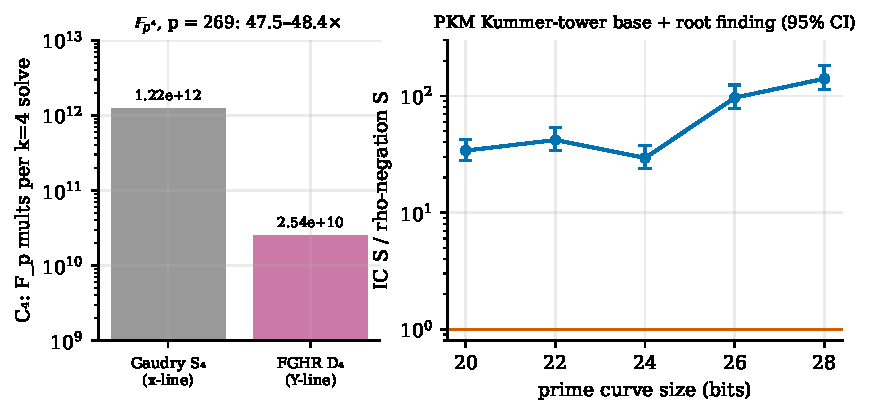
\includegraphics[width=\linewidth]{figures/fig-prime.pdf}
\caption[]{Left: cost $C_4$ of one $k=4$ decomposition over $\FF_{p^4}$,
$p=269$, Gaudry's $S_4$ system on the $x$-line against FGHR's $D_4$ system
on the $Y$-line (\art{research/gaudry_quartic_d4_20261013/}). Right:
index calculus with the PKM tower base and root finding over rho with
negation, eight one-target workloads $\times$ three rounds per size,
paired 95\% cluster-bootstrap intervals
(\art{research/pkm_tower_ecbench_20261013/}).}
\label{fig:prime}
\end{figure}
